\documentclass[1p]{elsarticle_modified}
%\bibliographystyle{elsarticle-num}

%\usepackage[colorlinks]{hyperref}
%\usepackage{abbrmath_seonhwa} %\Abb, \Ascr, \Acal ,\Abf, \Afrak
\usepackage{amsfonts}
\usepackage{amssymb}
\usepackage{amsmath}
\usepackage{amsthm}
\usepackage{scalefnt}
\usepackage{amsbsy}
\usepackage{kotex}
\usepackage{caption}
\usepackage{subfig}
\usepackage{color}
\usepackage{graphicx}
\usepackage{xcolor} %% white, black, red, green, blue, cyan, magenta, yellow
\usepackage{float}
\usepackage{setspace}
\usepackage{hyperref}

\usepackage{tikz}
\usetikzlibrary{arrows}

\usepackage{multirow}
\usepackage{array} % fixed length table
\usepackage{hhline}

%%%%%%%%%%%%%%%%%%%%%
\makeatletter
\renewcommand*\env@matrix[1][\arraystretch]{%
	\edef\arraystretch{#1}%
	\hskip -\arraycolsep
	\let\@ifnextchar\new@ifnextchar
	\array{*\c@MaxMatrixCols c}}
\makeatother %https://tex.stackexchange.com/questions/14071/how-can-i-increase-the-line-spacing-in-a-matrix
%%%%%%%%%%%%%%%

\usepackage[normalem]{ulem}

\newcommand{\msout}[1]{\ifmmode\text{\sout{\ensuremath{#1}}}\else\sout{#1}\fi}
%SOURCE: \msout is \stkout macro in https://tex.stackexchange.com/questions/20609/strikeout-in-math-mode

\newcommand{\cancel}[1]{
	\ifmmode
	{\color{red}\msout{#1}}
	\else
	{\color{red}\sout{#1}}
	\fi
}

\newcommand{\add}[1]{
	{\color{blue}\uwave{#1}}
}

\newcommand{\replace}[2]{
	\ifmmode
	{\color{red}\msout{#1}}{\color{blue}\uwave{#2}}
	\else
	{\color{red}\sout{#1}}{\color{blue}\uwave{#2}}
	\fi
}

\newcommand{\Sol}{\mathcal{S}} %segment
\newcommand{\D}{D} %diagram
\newcommand{\A}{\mathcal{A}} %arc


%%%%%%%%%%%%%%%%%%%%%%%%%%%%%5 test

\def\sl{\operatorname{\textup{SL}}(2,\Cbb)}
\def\psl{\operatorname{\textup{PSL}}(2,\Cbb)}
\def\quan{\mkern 1mu \triangleright \mkern 1mu}

\theoremstyle{definition}
\newtheorem{thm}{Theorem}[section]
\newtheorem{prop}[thm]{Proposition}
\newtheorem{lem}[thm]{Lemma}
\newtheorem{ques}[thm]{Question}
\newtheorem{cor}[thm]{Corollary}
\newtheorem{defn}[thm]{Definition}
\newtheorem{exam}[thm]{Example}
\newtheorem{rmk}[thm]{Remark}
\newtheorem{alg}[thm]{Algorithm}

\newcommand{\I}{\sqrt{-1}}
\begin{document}

%\begin{frontmatter}
%
%\title{Boundary parabolic representations of knots up to 8 crossings}
%
%%% Group authors per affiliation:
%\author{Yunhi Cho} 
%\address{Department of Mathematics, University of Seoul, Seoul, Korea}
%\ead{yhcho@uos.ac.kr}
%
%
%\author{Seonhwa Kim} %\fnref{s_kim}}
%\address{Center for Geometry and Physics, Institute for Basic Science, Pohang, 37673, Korea}
%\ead{ryeona17@ibs.re.kr}
%
%\author{Hyuk Kim}
%\address{Department of Mathematical Sciences, Seoul National University, Seoul 08826, Korea}
%\ead{hyukkim@snu.ac.kr}
%
%\author{Seokbeom Yoon}
%\address{Department of Mathematical Sciences, Seoul National University, Seoul, 08826,  Korea}
%\ead{sbyoon15@snu.ac.kr}
%
%\begin{abstract}
%We find all boundary parabolic representation of knots up to 8 crossings.
%
%\end{abstract}
%\begin{keyword}
%    \MSC[2010] 57M25 
%\end{keyword}
%
%\end{frontmatter}

%\linenumbers
%\tableofcontents
%
\newcommand\colored[1]{\textcolor{white}{\rule[-0.35ex]{0.8em}{1.4ex}}\kern-0.8em\color{red} #1}%
%\newcommand\colored[1]{\textcolor{white}{ #1}\kern-2.17ex	\textcolor{white}{ #1}\kern-1.81ex	\textcolor{white}{ #1}\kern-2.15ex\color{red}#1	}

{\Large $\underline{10_{100}~(K10a_{104})}$}

\setlength{\tabcolsep}{10pt}
\renewcommand{\arraystretch}{1.6}
\vspace{1cm}\begin{tabular}{m{100pt}>{\centering\arraybackslash}m{274pt}}
\multirow{5}{120pt}{
	\centering
	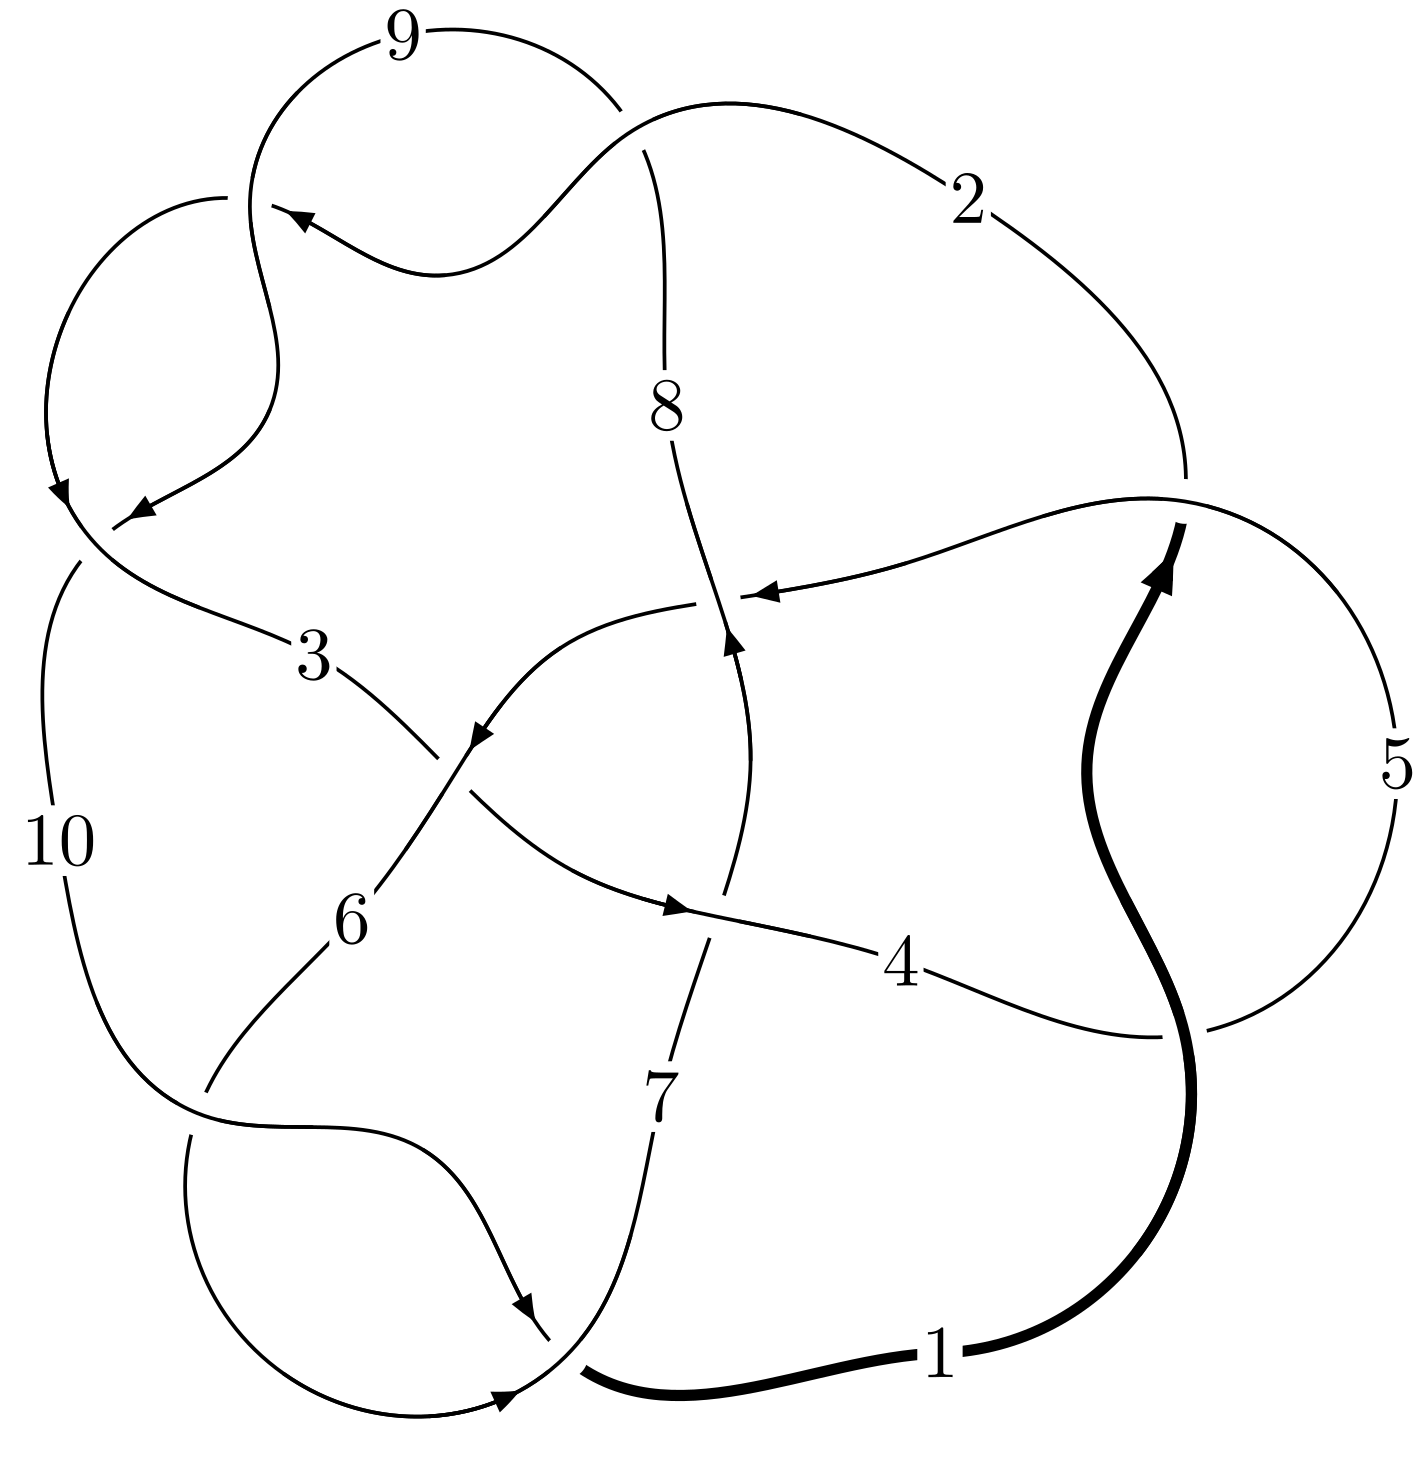
\includegraphics[width=112pt]{../../../GIT/diagram.site/Diagrams/png/184_10_100.png}\\
\ \ \ A knot diagram\footnotemark}&
\allowdisplaybreaks
\textbf{Linearized knot diagam} \\
\cline{2-2}
 &
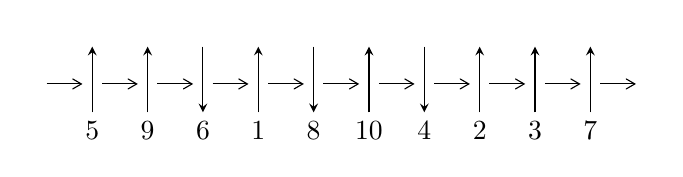
\begin{tikzpicture}[x=20pt, y=17pt]
	% nodes
	\node (C0) at (0, 0) {};
	\node (C1) at (1, 0) {};
	\node (C1U) at (1, +1) {};
	\node (C1D) at (1, -1) {5};

	\node (C2) at (2, 0) {};
	\node (C2U) at (2, +1) {};
	\node (C2D) at (2, -1) {9};

	\node (C3) at (3, 0) {};
	\node (C3U) at (3, +1) {};
	\node (C3D) at (3, -1) {6};

	\node (C4) at (4, 0) {};
	\node (C4U) at (4, +1) {};
	\node (C4D) at (4, -1) {1};

	\node (C5) at (5, 0) {};
	\node (C5U) at (5, +1) {};
	\node (C5D) at (5, -1) {8};

	\node (C6) at (6, 0) {};
	\node (C6U) at (6, +1) {};
	\node (C6D) at (6, -1) {10};

	\node (C7) at (7, 0) {};
	\node (C7U) at (7, +1) {};
	\node (C7D) at (7, -1) {4};

	\node (C8) at (8, 0) {};
	\node (C8U) at (8, +1) {};
	\node (C8D) at (8, -1) {2};

	\node (C9) at (9, 0) {};
	\node (C9U) at (9, +1) {};
	\node (C9D) at (9, -1) {3};

	\node (C10) at (10, 0) {};
	\node (C10U) at (10, +1) {};
	\node (C10D) at (10, -1) {7};
	\node (C11) at (11, 0) {};

	% arrows
	\draw[->,>={angle 60}]
	(C0) edge (C1) (C1) edge (C2) (C2) edge (C3) (C3) edge (C4) (C4) edge (C5) (C5) edge (C6) (C6) edge (C7) (C7) edge (C8) (C8) edge (C9) (C9) edge (C10) (C10) edge (C11) ;	\draw[->,>=stealth]
	(C1D) edge (C1U) (C2D) edge (C2U) (C3U) edge (C3D) (C4D) edge (C4U) (C5U) edge (C5D) (C6D) edge (C6U) (C7U) edge (C7D) (C8D) edge (C8U) (C9D) edge (C9U) (C10D) edge (C10U) ;
	\end{tikzpicture} \\
\hhline{~~} \\& 
\textbf{Solving Sequence} \\ \cline{2-2} 
 &
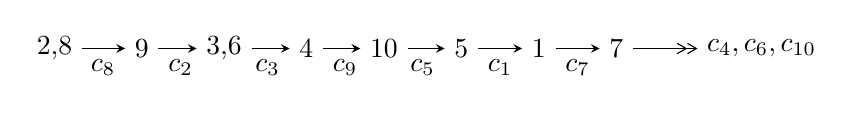
\begin{tikzpicture}[x=28pt, y=7pt]
	% node
	\node (A0) at (-1/8, 0) {2,8};
	\node (A1) at (1, 0) {9};
	\node (A2) at (33/16, 0) {3,6};
	\node (A3) at (25/8, 0) {4};
	\node (A4) at (33/8, 0) {10};
	\node (A5) at (41/8, 0) {5};
	\node (A6) at (49/8, 0) {1};
	\node (A7) at (57/8, 0) {7};
	\node (C1) at (1/2, -1) {$c_{8}$};
	\node (C2) at (3/2, -1) {$c_{2}$};
	\node (C3) at (21/8, -1) {$c_{3}$};
	\node (C4) at (29/8, -1) {$c_{9}$};
	\node (C5) at (37/8, -1) {$c_{5}$};
	\node (C6) at (45/8, -1) {$c_{1}$};
	\node (C7) at (53/8, -1) {$c_{7}$};
	\node (A8) at (9, 0) {$c_{4},c_{6},c_{10}$};

	% edge
	\draw[->,>=stealth]	
	(A0) edge (A1) (A1) edge (A2) (A2) edge (A3) (A3) edge (A4) (A4) edge (A5) (A5) edge (A6) (A6) edge (A7) ;
	\draw[->>,>={angle 60}]	
	(A7) edge (A8);
\end{tikzpicture} \\ 

\end{tabular} \\

\footnotetext{
The image of knot diagram is generated by the software ``\textbf{Draw programme}" developed by Andrew Bartholomew(\url{http://www.layer8.co.uk/maths/draw/index.htm\#Running-draw}), where we modified some parts for our purpose(\url{https://github.com/CATsTAILs/LinksPainter}).
}\phantom \\ \newline 
\centering \textbf{Ideals for irreducible components\footnotemark of $X_{\text{par}}$} 
 
\begin{align*}
I^u_{1}&=\langle 
-15 u^{13}+70 u^{12}+\cdots+2 b-42,\;49 u^{13}-224 u^{12}+\cdots+4 a+132,\\
\phantom{I^u_{1}}&\phantom{= \langle  }u^{14}-6 u^{13}+11 u^{12}-3 u^{11}- u^{10}-22 u^9+13 u^8+32 u^7-3 u^6-28 u^5-30 u^4+36 u^3+7 u^2-2 u-4\rangle \\
I^u_{2}&=\langle 
-1945 u^5 a^3+869 u^5 a^2+\cdots-1055 a-6821,\;- u^5 a^3+2 u^5 a^2+\cdots-14 a+22,\\
\phantom{I^u_{2}}&\phantom{= \langle  }u^6+u^5-3 u^4-2 u^3+2 u^2- u-1\rangle \\
I^u_{3}&=\langle 
- u^4+2 u^2+b,\;u^5-3 u^3+u^2+a+2 u-1,\;u^6- u^5-3 u^4+3 u^3+u^2- u+1\rangle \\
\\
\end{align*}
\raggedright * 3 irreducible components of $\dim_{\mathbb{C}}=0$, with total 44 representations.\\
\footnotetext{All coefficients of polynomials are rational numbers. But the coefficients are sometimes approximated in decimal forms when there is not enough margin.}
\newpage
\renewcommand{\arraystretch}{1}
\centering \section*{I. $I^u_{1}= \langle -15 u^{13}+70 u^{12}+\cdots+2 b-42,\;49 u^{13}-224 u^{12}+\cdots+4 a+132,\;u^{14}-6 u^{13}+\cdots-2 u-4 \rangle$}
\flushleft \textbf{(i) Arc colorings}\\
\begin{tabular}{m{7pt} m{180pt} m{7pt} m{180pt} }
\flushright $a_{2}=$&$\begin{pmatrix}0\\u\end{pmatrix}$ \\
\flushright $a_{8}=$&$\begin{pmatrix}1\\0\end{pmatrix}$ \\
\flushright $a_{9}=$&$\begin{pmatrix}1\\- u^2\end{pmatrix}$ \\
\flushright $a_{3}=$&$\begin{pmatrix}u\\- u^3+u\end{pmatrix}$ \\
\flushright $a_{6}=$&$\begin{pmatrix}-\frac{49}{4} u^{13}+56 u^{12}+\cdots-\frac{151}{4} u-33\\\frac{15}{2} u^{13}-35 u^{12}+\cdots+\frac{53}{2} u+21\end{pmatrix}$ \\
\flushright $a_{4}=$&$\begin{pmatrix}-\frac{7}{2} u^{13}+\frac{33}{2} u^{12}+\cdots-\frac{21}{2} u-\frac{21}{2}\\\frac{3}{2} u^{13}-7 u^{12}+\cdots+\frac{13}{2} u+4\end{pmatrix}$ \\
\flushright $a_{10}=$&$\begin{pmatrix}- u^2+1\\u^4-2 u^2\end{pmatrix}$ \\
\flushright $a_{5}=$&$\begin{pmatrix}-\frac{19}{4} u^{13}+21 u^{12}+\cdots-\frac{45}{4} u-12\\\frac{15}{2} u^{13}-35 u^{12}+\cdots+\frac{53}{2} u+21\end{pmatrix}$ \\
\flushright $a_{1}=$&$\begin{pmatrix}2 u^{13}-\frac{17}{2} u^{12}+\cdots+4 u+\frac{7}{2}\\-\frac{5}{2} u^{13}+12 u^{12}+\cdots-\frac{19}{2} u-8\end{pmatrix}$ \\
\flushright $a_{7}=$&$\begin{pmatrix}-\frac{3}{4} u^{13}+5 u^{12}+\cdots-\frac{21}{4} u-4\\-\frac{3}{2} u^{13}+6 u^{12}+\cdots-\frac{3}{2} u-3\end{pmatrix}$\\&\end{tabular}
\flushleft \textbf{(ii) Obstruction class $= -1$}\\~\\
\flushleft \textbf{(iii) Cusp Shapes $= -14 u^{13}+62 u^{12}-57 u^{11}-45 u^{10}-63 u^9+216 u^8+154 u^7-197 u^6-287 u^5-60 u^4+344 u^3+46 u^2-26 u-34$}\\~\\
\newpage\renewcommand{\arraystretch}{1}
\flushleft \textbf{(iv) u-Polynomials at the component}\newline \\
\begin{tabular}{m{50pt}|m{274pt}}
Crossings & \hspace{64pt}u-Polynomials at each crossing \\
\hline $$\begin{aligned}c_{1},c_{4},c_{6}\\c_{10}\end{aligned}$$&$\begin{aligned}
&u^{14}- u^{13}+\cdots-3 u+1
\end{aligned}$\\
\hline $$\begin{aligned}c_{2},c_{8},c_{9}\end{aligned}$$&$\begin{aligned}
&u^{14}-6 u^{13}+\cdots-2 u-4
\end{aligned}$\\
\hline $$\begin{aligned}c_{3},c_{5}\end{aligned}$$&$\begin{aligned}
&u^{14}+u^{13}+\cdots+5 u-1
\end{aligned}$\\
\hline $$\begin{aligned}c_{7}\end{aligned}$$&$\begin{aligned}
&u^{14}+14 u^{13}+\cdots-288 u-64
\end{aligned}$\\
\hline
\end{tabular}\\~\\
\newpage\renewcommand{\arraystretch}{1}
\flushleft \textbf{(v) Riley Polynomials at the component}\newline \\
\begin{tabular}{m{50pt}|m{274pt}}
Crossings & \hspace{64pt}Riley Polynomials at each crossing \\
\hline $$\begin{aligned}c_{1},c_{4},c_{6}\\c_{10}\end{aligned}$$&$\begin{aligned}
&y^{14}-13 y^{13}+\cdots-3 y+1
\end{aligned}$\\
\hline $$\begin{aligned}c_{2},c_{8},c_{9}\end{aligned}$$&$\begin{aligned}
&y^{14}-14 y^{13}+\cdots-60 y+16
\end{aligned}$\\
\hline $$\begin{aligned}c_{3},c_{5}\end{aligned}$$&$\begin{aligned}
&y^{14}+7 y^{13}+\cdots-59 y+1
\end{aligned}$\\
\hline $$\begin{aligned}c_{7}\end{aligned}$$&$\begin{aligned}
&y^{14}+2 y^{13}+\cdots-41984 y+4096
\end{aligned}$\\
\hline
\end{tabular}\\~\\
\newpage\flushleft \textbf{(vi) Complex Volumes and Cusp Shapes}
$$\begin{array}{c|c|c}  
\text{Solutions to }I^u_{1}& \I (\text{vol} + \sqrt{-1}CS) & \text{Cusp shape}\\
 \hline 
\begin{aligned}
u &= -1.04049\phantom{ +0.000000I} \\
a &= \phantom{-}0.567340\phantom{ +0.000000I} \\
b &= -1.20452\phantom{ +0.000000I}\end{aligned}
 & \phantom{-}0.339162\phantom{ +0.000000I} & \phantom{-}13.0620\phantom{ +0.000000I} \\ \hline\begin{aligned}
u &= -0.748785 + 0.823629 I \\
a &= \phantom{-}0.412890 - 0.456902 I \\
b &= \phantom{-}0.679306 + 1.137690 I\end{aligned}
 & \phantom{-}6.90977 - 8.77559 I & \phantom{-}9.73876 + 7.09449 I \\ \hline\begin{aligned}
u &= -0.748785 - 0.823629 I \\
a &= \phantom{-}0.412890 + 0.456902 I \\
b &= \phantom{-}0.679306 - 1.137690 I\end{aligned}
 & \phantom{-}6.90977 + 8.77559 I & \phantom{-}9.73876 - 7.09449 I \\ \hline\begin{aligned}
u &= -0.493094 + 1.098780 I \\
a &= -0.387144 - 0.128784 I \\
b &= \phantom{-}0.098682 - 0.905560 I\end{aligned}
 & \phantom{-}5.88215 + 2.52726 I & \phantom{-}13.28929 - 3.43101 I \\ \hline\begin{aligned}
u &= -0.493094 - 1.098780 I \\
a &= -0.387144 + 0.128784 I \\
b &= \phantom{-}0.098682 + 0.905560 I\end{aligned}
 & \phantom{-}5.88215 - 2.52726 I & \phantom{-}13.28929 + 3.43101 I \\ \hline\begin{aligned}
u &= \phantom{-}0.622591\phantom{ +0.000000I} \\
a &= \phantom{-}0.542539\phantom{ +0.000000I} \\
b &= \phantom{-}0.127481\phantom{ +0.000000I}\end{aligned}
 & \phantom{-}0.865875\phantom{ +0.000000I} & \phantom{-}12.3760\phantom{ +0.000000I} \\ \hline\begin{aligned}
u &= \phantom{-}1.45633 + 0.05562 I \\
a &= \phantom{-}0.38364 - 1.65172 I \\
b &= -0.429494 + 1.051770 I\end{aligned}
 & \phantom{-}4.42897 + 2.24150 I & \phantom{-}6.33861 - 3.08717 I \\ \hline\begin{aligned}
u &= \phantom{-}1.45633 - 0.05562 I \\
a &= \phantom{-}0.38364 + 1.65172 I \\
b &= -0.429494 - 1.051770 I\end{aligned}
 & \phantom{-}4.42897 - 2.24150 I & \phantom{-}6.33861 + 3.08717 I \\ \hline\begin{aligned}
u &= -0.303715 + 0.334799 I \\
a &= \phantom{-}0.003671 + 1.353790 I \\
b &= -0.729605 - 0.382323 I\end{aligned}
 & -1.31044 - 0.99980 I & -2.51765 + 3.01751 I \\ \hline\begin{aligned}
u &= -0.303715 - 0.334799 I \\
a &= \phantom{-}0.003671 - 1.353790 I \\
b &= -0.729605 + 0.382323 I\end{aligned}
 & -1.31044 + 0.99980 I & -2.51765 - 3.01751 I\\
 \hline 
 \end{array}$$\newpage$$\begin{array}{c|c|c}  
\text{Solutions to }I^u_{1}& \I (\text{vol} + \sqrt{-1}CS) & \text{Cusp shape}\\
 \hline 
\begin{aligned}
u &= \phantom{-}1.62071 + 0.25886 I \\
a &= -0.06147 + 1.67177 I \\
b &= \phantom{-}1.02771 - 1.53408 I\end{aligned}
 & \phantom{-}14.7349 + 12.8109 I & \phantom{-}11.37066 - 6.14968 I \\ \hline\begin{aligned}
u &= \phantom{-}1.62071 - 0.25886 I \\
a &= -0.06147 - 1.67177 I \\
b &= \phantom{-}1.02771 + 1.53408 I\end{aligned}
 & \phantom{-}14.7349 - 12.8109 I & \phantom{-}11.37066 + 6.14968 I \\ \hline\begin{aligned}
u &= \phantom{-}1.67750 + 0.35344 I \\
a &= -0.156526 - 0.920785 I \\
b &= -0.608077 + 1.061740 I\end{aligned}
 & \phantom{-}13.16540 + 3.07431 I & \phantom{-}13.56108 - 2.64554 I \\ \hline\begin{aligned}
u &= \phantom{-}1.67750 - 0.35344 I \\
a &= -0.156526 + 0.920785 I \\
b &= -0.608077 - 1.061740 I\end{aligned}
 & \phantom{-}13.16540 - 3.07431 I & \phantom{-}13.56108 + 2.64554 I\\
 \hline 
 \end{array}$$\newpage\newpage\renewcommand{\arraystretch}{1}
\centering \section*{II. $I^u_{2}= \langle -1945 u^5 a^3+869 u^5 a^2+\cdots-1055 a-6821,\;- u^5 a^3+2 u^5 a^2+\cdots-14 a+22,\;u^6+u^5-3 u^4-2 u^3+2 u^2- u-1 \rangle$}
\flushleft \textbf{(i) Arc colorings}\\
\begin{tabular}{m{7pt} m{180pt} m{7pt} m{180pt} }
\flushright $a_{2}=$&$\begin{pmatrix}0\\u\end{pmatrix}$ \\
\flushright $a_{8}=$&$\begin{pmatrix}1\\0\end{pmatrix}$ \\
\flushright $a_{9}=$&$\begin{pmatrix}1\\- u^2\end{pmatrix}$ \\
\flushright $a_{3}=$&$\begin{pmatrix}u\\- u^3+u\end{pmatrix}$ \\
\flushright $a_{6}=$&$\begin{pmatrix}a\\0.413566 a^{3} u^{5}-0.184776 a^{2} u^{5}+\cdots+0.224325 a+1.45035\end{pmatrix}$ \\
\flushright $a_{4}=$&$\begin{pmatrix}-0.321072 a^{3} u^{5}-0.0750585 a^{2} u^{5}+\cdots-0.0584733 a-1.19796\\0.0450776 a^{3} u^{5}-0.0967468 a^{2} u^{5}+\cdots+0.253243 a+0.104614\end{pmatrix}$ \\
\flushright $a_{10}=$&$\begin{pmatrix}- u^2+1\\u^4-2 u^2\end{pmatrix}$ \\
\flushright $a_{5}=$&$\begin{pmatrix}0.413566 a^{3} u^{5}-0.184776 a^{2} u^{5}+\cdots+1.22432 a+1.45035\\0.413566 a^{3} u^{5}-0.184776 a^{2} u^{5}+\cdots+0.224325 a+1.45035\end{pmatrix}$ \\
\flushright $a_{1}=$&$\begin{pmatrix}0.503934 a^{3} u^{5}-0.657027 a^{2} u^{5}+\cdots-0.0274293 a+2.75441\\0.182862 a^{3} u^{5}-0.732086 a^{2} u^{5}+\cdots-0.0859026 a+1.55645\end{pmatrix}$ \\
\flushright $a_{7}=$&$\begin{pmatrix}0.309802 a^{3} u^{5}-0.150755 a^{2} u^{5}+\cdots+1.24516 a+1.17181\\-0.0450776 a^{3} u^{5}+0.0967468 a^{2} u^{5}+\cdots-0.253243 a+0.895386\end{pmatrix}$\\&\end{tabular}
\flushleft \textbf{(ii) Obstruction class $= -1$}\\~\\
\flushleft \textbf{(iii) Cusp Shapes $= \frac{848}{4703} u^5 a^3-\frac{1820}{4703} u^5 a^2+\cdots+\frac{4764}{4703} a+\frac{48998}{4703}$}\\~\\
\newpage\renewcommand{\arraystretch}{1}
\flushleft \textbf{(iv) u-Polynomials at the component}\newline \\
\begin{tabular}{m{50pt}|m{274pt}}
Crossings & \hspace{64pt}u-Polynomials at each crossing \\
\hline $$\begin{aligned}c_{1},c_{4},c_{6}\\c_{10}\end{aligned}$$&$\begin{aligned}
&u^{24}+u^{23}+\cdots-8 u+1
\end{aligned}$\\
\hline $$\begin{aligned}c_{2},c_{8},c_{9}\end{aligned}$$&$\begin{aligned}
&(u^6+u^5-3 u^4-2 u^3+2 u^2- u-1)^4
\end{aligned}$\\
\hline $$\begin{aligned}c_{3},c_{5}\end{aligned}$$&$\begin{aligned}
&u^{24}-7 u^{23}+\cdots-372 u+73
\end{aligned}$\\
\hline $$\begin{aligned}c_{7}\end{aligned}$$&$\begin{aligned}
&(u^2- u+1)^{12}
\end{aligned}$\\
\hline
\end{tabular}\\~\\
\newpage\renewcommand{\arraystretch}{1}
\flushleft \textbf{(v) Riley Polynomials at the component}\newline \\
\begin{tabular}{m{50pt}|m{274pt}}
Crossings & \hspace{64pt}Riley Polynomials at each crossing \\
\hline $$\begin{aligned}c_{1},c_{4},c_{6}\\c_{10}\end{aligned}$$&$\begin{aligned}
&y^{24}-21 y^{23}+\cdots+72 y+1
\end{aligned}$\\
\hline $$\begin{aligned}c_{2},c_{8},c_{9}\end{aligned}$$&$\begin{aligned}
&(y^6-7 y^5+17 y^4-16 y^3+6 y^2-5 y+1)^4
\end{aligned}$\\
\hline $$\begin{aligned}c_{3},c_{5}\end{aligned}$$&$\begin{aligned}
&y^{24}+11 y^{23}+\cdots+52000 y+5329
\end{aligned}$\\
\hline $$\begin{aligned}c_{7}\end{aligned}$$&$\begin{aligned}
&(y^2+y+1)^{12}
\end{aligned}$\\
\hline
\end{tabular}\\~\\
\newpage\flushleft \textbf{(vi) Complex Volumes and Cusp Shapes}
$$\begin{array}{c|c|c}  
\text{Solutions to }I^u_{2}& \I (\text{vol} + \sqrt{-1}CS) & \text{Cusp shape}\\
 \hline 
\begin{aligned}
u &= \phantom{-}0.493180 + 0.575288 I \\
a &= \phantom{-}1.067300 - 0.316742 I \\
b &= -0.073003 - 0.780422 I\end{aligned}
 & \phantom{-}1.97456 - 0.05747 I & \phantom{-}6.57572 - 0.22068 I \\ \hline\begin{aligned}
u &= \phantom{-}0.493180 + 0.575288 I \\
a &= -0.584086 - 0.249616 I \\
b &= -0.678417 + 1.238260 I\end{aligned}
 & \phantom{-}1.97456 + 4.00229 I & \phantom{-}6.57572 - 7.14888 I \\ \hline\begin{aligned}
u &= \phantom{-}0.493180 + 0.575288 I \\
a &= \phantom{-}0.513478 + 1.284170 I \\
b &= \phantom{-}0.629282 - 0.637832 I\end{aligned}
 & \phantom{-}1.97456 + 4.00229 I & \phantom{-}6.57572 - 7.14888 I \\ \hline\begin{aligned}
u &= \phantom{-}0.493180 + 0.575288 I \\
a &= -0.136040 - 0.139388 I \\
b &= \phantom{-}0.617558 + 0.522759 I\end{aligned}
 & \phantom{-}1.97456 - 0.05747 I & \phantom{-}6.57572 - 0.22068 I \\ \hline\begin{aligned}
u &= \phantom{-}0.493180 - 0.575288 I \\
a &= \phantom{-}1.067300 + 0.316742 I \\
b &= -0.073003 + 0.780422 I\end{aligned}
 & \phantom{-}1.97456 + 0.05747 I & \phantom{-}6.57572 + 0.22068 I \\ \hline\begin{aligned}
u &= \phantom{-}0.493180 - 0.575288 I \\
a &= -0.584086 + 0.249616 I \\
b &= -0.678417 - 1.238260 I\end{aligned}
 & \phantom{-}1.97456 - 4.00229 I & \phantom{-}6.57572 + 7.14888 I \\ \hline\begin{aligned}
u &= \phantom{-}0.493180 - 0.575288 I \\
a &= \phantom{-}0.513478 - 1.284170 I \\
b &= \phantom{-}0.629282 + 0.637832 I\end{aligned}
 & \phantom{-}1.97456 - 4.00229 I & \phantom{-}6.57572 + 7.14888 I \\ \hline\begin{aligned}
u &= \phantom{-}0.493180 - 0.575288 I \\
a &= -0.136040 + 0.139388 I \\
b &= \phantom{-}0.617558 - 0.522759 I\end{aligned}
 & \phantom{-}1.97456 + 0.05747 I & \phantom{-}6.57572 + 0.22068 I \\ \hline\begin{aligned}
u &= -0.483672\phantom{ +0.000000I} \\
a &= \phantom{-}1.44157 + 0.74757 I \\
b &= \phantom{-}1.09154 - 1.08035 I\end{aligned}
 & \phantom{-}5.67365 - 2.02988 I & \phantom{-}15.4168 + 3.4641 I \\ \hline\begin{aligned}
u &= -0.483672\phantom{ +0.000000I} \\
a &= \phantom{-}1.44157 - 0.74757 I \\
b &= \phantom{-}1.09154 + 1.08035 I\end{aligned}
 & \phantom{-}5.67365 + 2.02988 I & \phantom{-}15.4168 - 3.4641 I\\
 \hline 
 \end{array}$$\newpage$$\begin{array}{c|c|c}  
\text{Solutions to }I^u_{2}& \I (\text{vol} + \sqrt{-1}CS) & \text{Cusp shape}\\
 \hline 
\begin{aligned}
u &= -0.483672\phantom{ +0.000000I} \\
a &= -2.95401 + 1.87206 I \\
b &= -0.006188 - 0.799526 I\end{aligned}
 & \phantom{-}5.67365 - 2.02988 I & \phantom{-}15.4168 + 3.4641 I \\ \hline\begin{aligned}
u &= -0.483672\phantom{ +0.000000I} \\
a &= -2.95401 - 1.87206 I \\
b &= -0.006188 + 0.799526 I\end{aligned}
 & \phantom{-}5.67365 + 2.02988 I & \phantom{-}15.4168 - 3.4641 I \\ \hline\begin{aligned}
u &= -1.52087 + 0.16310 I \\
a &= \phantom{-}0.299570 - 1.150850 I \\
b &= \phantom{-}0.618593 + 0.988703 I\end{aligned}
 & \phantom{-}8.63038 - 2.56224 I & \phantom{-}10.58114 - 0.25928 I \\ \hline\begin{aligned}
u &= -1.52087 + 0.16310 I \\
a &= -0.601099 + 1.113320 I \\
b &= \phantom{-}0.554158 - 1.044580 I\end{aligned}
 & \phantom{-}8.63038 - 2.56224 I & \phantom{-}10.58114 - 0.25928 I \\ \hline\begin{aligned}
u &= -1.52087 + 0.16310 I \\
a &= -0.07073 - 1.79722 I \\
b &= \phantom{-}0.427101 + 0.945943 I\end{aligned}
 & \phantom{-}8.63038 - 6.62201 I & \phantom{-}10.58114 + 6.66892 I \\ \hline\begin{aligned}
u &= -1.52087 + 0.16310 I \\
a &= \phantom{-}0.18899 + 2.07712 I \\
b &= -1.06187 - 1.93363 I\end{aligned}
 & \phantom{-}8.63038 - 6.62201 I & \phantom{-}10.58114 + 6.66892 I \\ \hline\begin{aligned}
u &= -1.52087 - 0.16310 I \\
a &= \phantom{-}0.299570 + 1.150850 I \\
b &= \phantom{-}0.618593 - 0.988703 I\end{aligned}
 & \phantom{-}8.63038 + 2.56224 I & \phantom{-}10.58114 + 0.25928 I \\ \hline\begin{aligned}
u &= -1.52087 - 0.16310 I \\
a &= -0.601099 - 1.113320 I \\
b &= \phantom{-}0.554158 + 1.044580 I\end{aligned}
 & \phantom{-}8.63038 + 2.56224 I & \phantom{-}10.58114 + 0.25928 I \\ \hline\begin{aligned}
u &= -1.52087 - 0.16310 I \\
a &= -0.07073 + 1.79722 I \\
b &= \phantom{-}0.427101 - 0.945943 I\end{aligned}
 & \phantom{-}8.63038 + 6.62201 I & \phantom{-}10.58114 - 6.66892 I \\ \hline\begin{aligned}
u &= -1.52087 - 0.16310 I \\
a &= \phantom{-}0.18899 - 2.07712 I \\
b &= -1.06187 + 1.93363 I\end{aligned}
 & \phantom{-}8.63038 + 6.62201 I & \phantom{-}10.58114 - 6.66892 I\\
 \hline 
 \end{array}$$\newpage$$\begin{array}{c|c|c}  
\text{Solutions to }I^u_{2}& \I (\text{vol} + \sqrt{-1}CS) & \text{Cusp shape}\\
 \hline 
\begin{aligned}
u &= \phantom{-}1.53904\phantom{ +0.000000I} \\
a &= -0.49479 + 1.36564 I \\
b &= -0.628935 - 0.898287 I\end{aligned}
 & \phantom{-}12.59490 - 2.02988 I & \phantom{-}14.2695 + 3.4641 I \\ \hline\begin{aligned}
u &= \phantom{-}1.53904\phantom{ +0.000000I} \\
a &= -0.49479 - 1.36564 I \\
b &= -0.628935 + 0.898287 I\end{aligned}
 & \phantom{-}12.59490 + 2.02988 I & \phantom{-}14.2695 - 3.4641 I \\ \hline\begin{aligned}
u &= \phantom{-}1.53904\phantom{ +0.000000I} \\
a &= -1.17015 + 1.51812 I \\
b &= \phantom{-}2.01019 - 1.49411 I\end{aligned}
 & \phantom{-}12.59490 - 2.02988 I & \phantom{-}14.2695 + 3.4641 I \\ \hline\begin{aligned}
u &= \phantom{-}1.53904\phantom{ +0.000000I} \\
a &= -1.17015 - 1.51812 I \\
b &= \phantom{-}2.01019 + 1.49411 I\end{aligned}
 & \phantom{-}12.59490 + 2.02988 I & \phantom{-}14.2695 - 3.4641 I\\
 \hline 
 \end{array}$$\newpage\newpage\renewcommand{\arraystretch}{1}
\centering \section*{III. $I^u_{3}= \langle - u^4+2 u^2+b,\;u^5-3 u^3+u^2+a+2 u-1,\;u^6- u^5-3 u^4+3 u^3+u^2- u+1 \rangle$}
\flushleft \textbf{(i) Arc colorings}\\
\begin{tabular}{m{7pt} m{180pt} m{7pt} m{180pt} }
\flushright $a_{2}=$&$\begin{pmatrix}0\\u\end{pmatrix}$ \\
\flushright $a_{8}=$&$\begin{pmatrix}1\\0\end{pmatrix}$ \\
\flushright $a_{9}=$&$\begin{pmatrix}1\\- u^2\end{pmatrix}$ \\
\flushright $a_{3}=$&$\begin{pmatrix}u\\- u^3+u\end{pmatrix}$ \\
\flushright $a_{6}=$&$\begin{pmatrix}- u^5+3 u^3- u^2-2 u+1\\u^4-2 u^2\end{pmatrix}$ \\
\flushright $a_{4}=$&$\begin{pmatrix}u^5-3 u^3+2 u\\- u^3+2 u\end{pmatrix}$ \\
\flushright $a_{10}=$&$\begin{pmatrix}- u^2+1\\u^4-2 u^2\end{pmatrix}$ \\
\flushright $a_{5}=$&$\begin{pmatrix}- u^5+u^4+3 u^3-3 u^2-2 u+1\\u^4-2 u^2\end{pmatrix}$ \\
\flushright $a_{1}=$&$\begin{pmatrix}u^5- u^4-4 u^3+3 u^2+3 u-1\\u^5-3 u^3+u^2+2 u-1\end{pmatrix}$ \\
\flushright $a_{7}=$&$\begin{pmatrix}- u^5+u^4+3 u^3-3 u^2-2 u+2\\- u^5+u^4+3 u^3-3 u^2- u+1\end{pmatrix}$\\&\end{tabular}
\flushleft \textbf{(ii) Obstruction class $= 1$}\\~\\
\flushleft \textbf{(iii) Cusp Shapes $= -4 u^5+2 u^4+8 u^3-4 u^2+3 u+7$}\\~\\
\newpage\renewcommand{\arraystretch}{1}
\flushleft \textbf{(iv) u-Polynomials at the component}\newline \\
\begin{tabular}{m{50pt}|m{274pt}}
Crossings & \hspace{64pt}u-Polynomials at each crossing \\
\hline $$\begin{aligned}c_{1},c_{6}\end{aligned}$$&$\begin{aligned}
&u^6- u^5-3 u^4+3 u^3+3 u^2-3 u-1
\end{aligned}$\\
\hline $$\begin{aligned}c_{2}\end{aligned}$$&$\begin{aligned}
&u^6+u^5-3 u^4-3 u^3+u^2+u+1
\end{aligned}$\\
\hline $$\begin{aligned}c_{3},c_{5}\end{aligned}$$&$\begin{aligned}
&u^6+u^5+u^4+u^3- u^2- u-1
\end{aligned}$\\
\hline $$\begin{aligned}c_{4},c_{10}\end{aligned}$$&$\begin{aligned}
&u^6+u^5-3 u^4-3 u^3+3 u^2+3 u-1
\end{aligned}$\\
\hline $$\begin{aligned}c_{7}\end{aligned}$$&$\begin{aligned}
&u^6- u^5+u^4+u^3- u^2+u-1
\end{aligned}$\\
\hline $$\begin{aligned}c_{8},c_{9}\end{aligned}$$&$\begin{aligned}
&u^6- u^5-3 u^4+3 u^3+u^2- u+1
\end{aligned}$\\
\hline
\end{tabular}\\~\\
\newpage\renewcommand{\arraystretch}{1}
\flushleft \textbf{(v) Riley Polynomials at the component}\newline \\
\begin{tabular}{m{50pt}|m{274pt}}
Crossings & \hspace{64pt}Riley Polynomials at each crossing \\
\hline $$\begin{aligned}c_{1},c_{4},c_{6}\\c_{10}\end{aligned}$$&$\begin{aligned}
&y^6-7 y^5+21 y^4-35 y^3+33 y^2-15 y+1
\end{aligned}$\\
\hline $$\begin{aligned}c_{2},c_{8},c_{9}\end{aligned}$$&$\begin{aligned}
&y^6-7 y^5+17 y^4-15 y^3+y^2+y+1
\end{aligned}$\\
\hline $$\begin{aligned}c_{3},c_{5}\end{aligned}$$&$\begin{aligned}
&y^6+y^5-3 y^4-3 y^3+y^2+y+1
\end{aligned}$\\
\hline $$\begin{aligned}c_{7}\end{aligned}$$&$\begin{aligned}
&y^6+y^5+y^4-3 y^3-3 y^2+y+1
\end{aligned}$\\
\hline
\end{tabular}\\~\\
\newpage\flushleft \textbf{(vi) Complex Volumes and Cusp Shapes}
$$\begin{array}{c|c|c}  
\text{Solutions to }I^u_{3}& \I (\text{vol} + \sqrt{-1}CS) & \text{Cusp shape}\\
 \hline 
\begin{aligned}
u &= -0.847445\phantom{ +0.000000I} \\
a &= \phantom{-}0.587994\phantom{ +0.000000I} \\
b &= -0.920568\phantom{ +0.000000I}\end{aligned}
 & -0.285060\phantom{ +0.000000I} & -0.503990\phantom{ +0.000000I} \\ \hline\begin{aligned}
u &= \phantom{-}0.251489 + 0.528716 I \\
a &= \phantom{-}0.07352 - 1.42421 I \\
b &= \phantom{-}0.408651 - 0.646904 I\end{aligned}
 & \phantom{-}4.59420 - 1.63935 I & \phantom{-}6.79257 + 0.07886 I \\ \hline\begin{aligned}
u &= \phantom{-}0.251489 - 0.528716 I \\
a &= \phantom{-}0.07352 + 1.42421 I \\
b &= \phantom{-}0.408651 + 0.646904 I\end{aligned}
 & \phantom{-}4.59420 + 1.63935 I & \phantom{-}6.79257 - 0.07886 I \\ \hline\begin{aligned}
u &= \phantom{-}1.46321 + 0.18726 I \\
a &= -0.71355 - 1.48541 I \\
b &= -0.077247 + 1.212100 I\end{aligned}
 & \phantom{-}9.23208 + 4.33255 I & \phantom{-}12.59516 - 4.05038 I \\ \hline\begin{aligned}
u &= \phantom{-}1.46321 - 0.18726 I \\
a &= -0.71355 + 1.48541 I \\
b &= -0.077247 - 1.212100 I\end{aligned}
 & \phantom{-}9.23208 - 4.33255 I & \phantom{-}12.59516 + 4.05038 I \\ \hline\begin{aligned}
u &= -1.58196\phantom{ +0.000000I} \\
a &= -0.307931\phantom{ +0.000000I} \\
b &= \phantom{-}1.25776\phantom{ +0.000000I}\end{aligned}
 & \phantom{-}12.1109\phantom{ +0.000000I} & \phantom{-}12.7290\phantom{ +0.000000I}\\
 \hline 
 \end{array}$$\newpage
\newpage\renewcommand{\arraystretch}{1}
\centering \section*{ IV. u-Polynomials}
\begin{tabular}{m{50pt}|m{274pt}}
Crossings & \hspace{64pt}u-Polynomials at each crossing \\
\hline $$\begin{aligned}c_{1},c_{6}\end{aligned}$$&$\begin{aligned}
&(u^6- u^5-3 u^4+3 u^3+3 u^2-3 u-1)(u^{14}- u^{13}+\cdots-3 u+1)\\
&\cdot(u^{24}+u^{23}+\cdots-8 u+1)
\end{aligned}$\\
\hline $$\begin{aligned}c_{2}\end{aligned}$$&$\begin{aligned}
&(u^6+u^5-3 u^4-3 u^3+u^2+u+1)(u^6+u^5-3 u^4-2 u^3+2 u^2- u-1)^{4}\\
&\cdot(u^{14}-6 u^{13}+\cdots-2 u-4)
\end{aligned}$\\
\hline $$\begin{aligned}c_{3},c_{5}\end{aligned}$$&$\begin{aligned}
&(u^6+u^5+u^4+u^3- u^2- u-1)(u^{14}+u^{13}+\cdots+5 u-1)\\
&\cdot(u^{24}-7 u^{23}+\cdots-372 u+73)
\end{aligned}$\\
\hline $$\begin{aligned}c_{4},c_{10}\end{aligned}$$&$\begin{aligned}
&(u^6+u^5-3 u^4-3 u^3+3 u^2+3 u-1)(u^{14}- u^{13}+\cdots-3 u+1)\\
&\cdot(u^{24}+u^{23}+\cdots-8 u+1)
\end{aligned}$\\
\hline $$\begin{aligned}c_{7}\end{aligned}$$&$\begin{aligned}
&(u^2- u+1)^{12}(u^6- u^5+u^4+u^3- u^2+u-1)\\
&\cdot(u^{14}+14 u^{13}+\cdots-288 u-64)
\end{aligned}$\\
\hline $$\begin{aligned}c_{8},c_{9}\end{aligned}$$&$\begin{aligned}
&(u^6- u^5-3 u^4+3 u^3+u^2- u+1)(u^6+u^5-3 u^4-2 u^3+2 u^2- u-1)^{4}\\
&\cdot(u^{14}-6 u^{13}+\cdots-2 u-4)
\end{aligned}$\\
\hline
\end{tabular}\newpage\renewcommand{\arraystretch}{1}
\centering \section*{ V. Riley Polynomials}
\begin{tabular}{m{50pt}|m{274pt}}
Crossings & \hspace{64pt}Riley Polynomials at each crossing \\
\hline $$\begin{aligned}c_{1},c_{4},c_{6}\\c_{10}\end{aligned}$$&$\begin{aligned}
&(y^6-7 y^5+\cdots-15 y+1)(y^{14}-13 y^{13}+\cdots-3 y+1)\\
&\cdot(y^{24}-21 y^{23}+\cdots+72 y+1)
\end{aligned}$\\
\hline $$\begin{aligned}c_{2},c_{8},c_{9}\end{aligned}$$&$\begin{aligned}
&(y^6-7 y^5+17 y^4-16 y^3+6 y^2-5 y+1)^4\\
&\cdot(y^6-7 y^5+\cdots+y+1)(y^{14}-14 y^{13}+\cdots-60 y+16)
\end{aligned}$\\
\hline $$\begin{aligned}c_{3},c_{5}\end{aligned}$$&$\begin{aligned}
&(y^6+y^5-3 y^4-3 y^3+y^2+y+1)(y^{14}+7 y^{13}+\cdots-59 y+1)\\
&\cdot(y^{24}+11 y^{23}+\cdots+52000 y+5329)
\end{aligned}$\\
\hline $$\begin{aligned}c_{7}\end{aligned}$$&$\begin{aligned}
&(y^2+y+1)^{12}(y^6+y^5+y^4-3 y^3-3 y^2+y+1)\\
&\cdot(y^{14}+2 y^{13}+\cdots-41984 y+4096)
\end{aligned}$\\
\hline
\end{tabular}
\vskip 2pc
\end{document}